%-------------------------
%big-picture
%(c) H.Buchmann FHNW 2019
%export TEXINPUTS=${HOME}/fhnw/edu/:${HOME}/fhnw/edu/tinL/config/latex:${HOME}/fhnw/edu/config//:
%-------------------------
\documentclass{beamer}
\usepackage{latex/beamer}
%---------------------
%local defines
%(c) H.Buchmann FHNW 2009
%$Id$
%---------------------
\newcommand{\target} {\beaglebone\xspace}
\newcommand{\targetS}{{\bf BBG}\xspace}
\newcommand{\host}   {{\em Host}\xspace}
\newcommand{\targetroot} {{\bf target-root}\xspace}
\newcommand{\kernel} {{\bf kernel}\xspace}
\renewcommand{\c}{{\bf C}\xspace}
\newcommand{\cpp}{{\bf C++}\xspace}
\newcommand{\posix}{{\bf POSIX}\xspace}


\title[Crossdevelopment]{Crossdevelopment}
\begin{document}

\frame{\titlepage}

\begin{frame}{Entwicklung von Programmen auf dem \target}
 \begin{block}{Nicht aus den Augen verlieren:}
 \begin{itemize}
  \item alles ist ein File 
  \begin{itemize}
   \item $0-te$ Näherung
   \item File: {\em stream of bits}
   \item wo sind die Files ?
  \end{itemize}
  \item Filesysteme
  \begin{itemize}
   \item \cod{mount}
   \item \cod{sshfs}
  \end{itemize}
  \item Cross development
  \begin{itemize}
   \item \host $\leftrightarrow$ \target
   \remark{Keine Toolchain auf dem \target}
  \end{itemize}
 \end{itemize}
 \end{block}
\end{frame}

\begin{frame}{Wichtig}
 \begin{itemize}
  \item wo ist was ?
  \begin{itemize}
  \item {\Large Verzeichnisstruktur}
  \end{itemize}
  \item wo sind wir ?
  \begin{itemize}
   \item \host
   \item[] oder
   \item \target
  \end{itemize}
 \end{itemize}
\end{frame}

\begin{frame}{Ein paar Befehle}
 \begin{itemize}
  \item \cod{cat {\em name}} 
  \begin{itemize}
   \item {\em concatenate files and print on the standard output}
  \end{itemize}
  \item \cod{hexdump -C {\em name}}
  \begin{itemize}
   \item {\em display  file  contents  in hexadecimal, decimal, octal, or ascii}
  \end{itemize}
  \item \cod{dd if=... of=... count=...}
  \begin{itemize}
   \item {\em convert and copy a file}
  \end{itemize}
  \item \cod{cp}
  \begin{itemize}
   \item {\em copy files and directories}
  \end{itemize}
   \item \cod{rsync}
  \begin{itemize}
   \item {\em a fast, versatile, remote (and local) file-copying tool}
  \end{itemize}
  \item \cod{tar}
  \begin{itemize}
   \item {\em archiving utility}
  \end{itemize}
 \end{itemize}
\end{frame}

\begin{frame}{Devices sind auch Files}
 \begin{itemize}
  \item SD-Karten \cod{/dev/sd{\bf X}}
  \item serielle Schnittstellen \cod{/dev/tty{\bf X}}
  \begin{itemize}
   \item \cod{/dev/ttyUSB0} \cod{/dev/ttyACM0}
  \end{itemize}
  \item $\dots$
 \end{itemize}
 
\end{frame}

%\section{Cross development}
\section{CrossDevelopment}
\begin{frame}{Crossdevelopment}
 \begin{itemize}
  \item zwei Rechner
  \begin{description}
   \item[Host] der Entwicklungsrechner
   \item[Target] \targetS der Zielrechner
  \end{description}
  \item Development
  \begin{itemize}
   \item Wo sind die Files
  \end{itemize}
  \item CrossDevelopment
  \begin{itemize}
   \item Wo sind die Files
  \end{itemize}
 \end{itemize}
\end{frame}

\subsection{Outline}
\begin{frame}{Outline}
 \begin{itemize}
  \item Development
  \begin{itemize}
   \item Programme auf dem \host für den \host
  \end{itemize}
  \item CrossDevelopment
  \begin{itemize}
   \item Programme auf dem \host für für den \target
  \end{itemize}
 \end{itemize}
\end{frame}

\begin{frame}{Verzeichnisstruktur}
 \dirtree{%
 .1 6-crossdevelopment.
 .2 src \DTcomment{the source files}.
 .2 tc \DTcomment{target toolchain normally link}.
 .2 target-work \DTcomment{files for \targetS}.
 .2 host-work \DTcomment{files for \host}.
 .2 target-root \DTcomment{copy from SD-card $|$ link $|$ mounted}.
 }
\end{frame}

\subsection{Development}

\begin{frame}{Development (noch nicht Cross):Verzeichnis: \cod{host-work}}{die einzelnen Schritte}
 \begin{itemize}
  \item Source file \cod{src/hello-world.cc}
  \begin{itemize}
   \item C++/POSIX
  \end{itemize}
  unabhängig von Platform
  \item Object file (Maschinencode) \cod{hello-world.o}
  \begin{itemize}
   \item erzeugt mit: \cod{g++ -c ../src/hello-world.cc -o hello-world.o}
   \item Maschinencode: 
   \begin{itemize}
    \item \cod{file hello-world.o} 
    \item \cod{objdump -d hello-world.o}
   \end{itemize}
  \end{itemize}
  \item Executable file \cod{hello-world}
  \begin{itemize}
   \item \cod{g++  hello-world.o -o hello-world}
   \item Maschinencode:
   \begin{itemize}
    \item \cod{file hello-world-c} 
    \item \cod{objdump -d hello-world-c}
   \end{itemize}
  \end{itemize}
 \end{itemize}
\end{frame}

\begin{frame}{In einem Schritt}{für kleine Projekte}
 \begin{itemize}
  \item \cod{g++ ../src/hello-world.cc -o hello-world}
 \end{itemize}
\end{frame}

\begin{frame}{Was es braucht ?}{Files}
 \begin{itemize}
  \item Source file
  \begin{itemize}
   \item wo ist der {\em include file} \cod{iostream}
  \end{itemize}
  \item Object File
  \begin{itemize}
   \item \cod{nm hello-world.o}
   \item wo ist z.B. \cod{\_ZSt4cout}
  \end{itemize}
  \item Executable
  \begin{itemize}
  \item \cod{nm hello-world}
  \item \cod{ldd hello-world}
  \item wo sind die Bibliotheken
  \end{itemize}
 \end{itemize}
\end{frame}

\begin{frame}{Wo sind die Files ?}{irgendwo in einem Unterverzeichnis von {\Huge\tt /}}
 \begin{itemize}
  \item Include Files \cod{g++  -v ../src/hello-world.cc -o hello-world}
  \begin{itemize}
   \item \cod{iostream} ?
  \end{itemize}
  \item Bibliotheken
  \begin{itemize}
   \item z.B. \cod{libc.so}
  \end{itemize}
 \end{itemize}
\end{frame}

\begin{frame}{Development}
 \begin{itemize}
  \item Host==Target
  \item root Host==root Target
 \end{itemize}
\end{frame}

\subsection{CrossDevelopment}

\begin{frame}{CrossDevelopment}
 \begin{itemize}
  \item Host!=Target
  \item root Host != root Target
 \end{itemize}
\end{frame}



\begin{frame}{CrossDevelopment}{Target \target}
 \begin{itemize}
  \item toolchain
  \begin{itemize}
   \item \cod{tc/bin/arm-linux-gnueabihf-*}
   \item \cod{*}: \cod{g++},\cod{nm},\cod{objdump} $\dots$
  \end{itemize}
  \item \cod{target-root} Mehrere Möglichkeiten:
  \begin{itemize}
   \item Kopie von SD-Karte 
   \item \cod{sshfs debian@192.168.7.2:/ target-root}
  \end{itemize}
 \end{itemize}
\end{frame}

\begin{frame}{CrossDevelopment: im Verzeichnis \cod{target-work}}{die einzelnen Schritte}
 \begin{itemize}
  \item Source file \cod{src/hello-world.cc}
  \begin{itemize}
   \item C++/POSIX
  \end{itemize}
  unabhängig von Platform
  \item Object file (Maschinencode) \cod{hello-world.o}
  \begin{itemize}
   \item erzeugt mit: \cod{../tc/bin/arm-linux-gnueabihf-g++ --sysroot=../target-root -c ../src/hello-world.cc -o hello-world.o}
   \item Maschinencode: 
   \begin{itemize}
    \item \cod{file hello-world.o} 
    \item \cod{../tc/bin/arm-linux-gnueabihf-objdump -d hello-world.o}
   \end{itemize}
  \end{itemize}
  \item Executable file \cod{hello-world}
  \begin{itemize}
   \item \cod{../tc/bin/arm-linux-gnueabihf-g++ --sysroot=../target-root hello-world.o -o hello-world}
   \item Maschinencode:
   \begin{itemize}
    \item \cod{file hello-world-c} 
    \item \cod{../tc/bin/arm-linux-gnueabihf-objdump -d hello-world-c}
   \end{itemize}
  \end{itemize}
 \end{itemize}
\end{frame}

\begin{frame}{In einem Schritt}{für kleine Projekte}
 \begin{itemize}
  \item \cod{../tc/bin/arm-linux-gnueabihf-g++ --sysroot=../target-root ../src/hello-world.cc -o hello-world}
 \end{itemize}
\end{frame}


%\subsection{Development}
%
%\begin{frame}{Development}{noch nicht Cross}
% \begin{itemize}
%  \item Source file \cod{src/hello-world-c.c}
%  \begin{itemize}
%   \item C
%   \item POSIX
%  \end{itemize}
%  unabhängig von Platform
%  \item Object file (Maschinencode) \cod{hello-world-c.o}
%  \begin{itemize}
%   \item erzeugt mit: \cod{gcc -c ../src/hello-world-c.c -o hello-world-c.o}
%   \item Maschinencode: 
%   \begin{itemize}
%    \item \cod{file hello-world-c.o} 
%    \item \cod{objdump -d hello-world-c.o}
%   \end{itemize}
%  \end{itemize}
%  \item Executable file \cod{hello-world-c}
%  \begin{itemize}
%   \item \cod{gcc  hello-world-c.o -o hello-world-c}
%   \item Maschinencode:
%   \begin{itemize}
%    \item \cod{file hello-world-c} 
%    \item \cod{objdump -d hello-world-c}
%   \end{itemize}
%  \end{itemize}
% \end{itemize}
%\end{frame}
%
%\begin{frame}{Was es braucht ?}{Files}
% \begin{itemize}
%  \item Source file
%  \begin{itemize}
%   \item wo ist der {\em include file} \cod{stdio.h}
%  \end{itemize}
%  \item Object File
%  \begin{itemize}
%   \item \cod{nm hello-world-c.o}
%   \item wo ist \cod{puts}
%  \end{itemize}
%  \item Executable
%  \begin{itemize}
%  \item \cod{nm hello-world-c}
%  \item \cod{ldd hello-world-c}
%  \item wo sind die Bibliotheken
%  \end{itemize}
% \end{itemize}
%\end{frame}
%
%\begin{frame}{Wo sind die Files ?}{irgendwo in einem Unterverzeichnis von {\Huge\tt /}}
% \begin{itemize}
%  \item Include Files \cod{gcc -c -v ../src/hello-world-c.c -o hello-world-c.o}
%  \begin{itemize}
%   \item \cod{stdio.h} ?
%   \item \cod{stddef.h} ? 
%  \end{itemize}
%  \item Bibliotheken
%  \begin{itemize}
%   \item z.B. \cod{libc.so}
%  \end{itemize}
% \end{itemize}
%\end{frame}
%
%\begin{frame}{Development}{der Normalfall}
% \begin{itemize}
%  \item Host==Target
%  \item root Host==root Target
% \end{itemize}
%\end{frame}


%%-------------------------
%minimal-unix
%(c) H.Buchmann FHNW 2014
%export TEXINPUTS=${HOME}/fhnw/edu/:${HOME}/fhnw/edu/tinL/config/latex:${HOME}/fhnw/edu/config//:
%-------------------------
\documentclass{beamer}
\usepackage{latex/beamer}
%---------------------
%local defines
%(c) H.Buchmann FHNW 2009
%$Id$
%---------------------
\newcommand{\target} {\beaglebone\xspace}
\newcommand{\targetS}{{\bf BBG}\xspace}
\newcommand{\host}   {{\em Host}\xspace}
\newcommand{\targetroot} {{\bf target-root}\xspace}
\newcommand{\kernel} {{\bf kernel}\xspace}
\renewcommand{\c}{{\bf C}\xspace}
\newcommand{\cpp}{{\bf C++}\xspace}
\newcommand{\posix}{{\bf POSIX}\xspace}

\input{/home/buchmann/latex/dirtree/dirtree.tex}

\usepackage[absolute]{textpos}
\setlength{\TPHorizModule}{1mm}
\setlength{\TPVertModule}{1mm}

\begin{document}

\newcommand{\qemu}{{\em qemu}\xspace}
\newcommand{\busybox}{{\em busybox}\xspace}
\newcommand{\yocto}{{\em yocto}\xspace}
\title{Zugriff auf die Hardware}

\frame{\titlepage}

\begin{frame}{Um was geht es ?}{Zugriff auf mehrere Arten}
 \begin{itemize}
  \item userspace
  \begin{itemize}
   \item per \cod{/sys/class/gpio}
   \item per \cod{mmap} mit eigenem Programm: 
  \end{itemize}
  \item kernelspace
  \begin{itemize}
   \item mit eigenem module
  \end{itemize}
 \end{itemize}
\end{frame}

\section{Userspace}
\subsection{sys/class/gpio}
\begin{frame}{\cod{sys/class/gpio}}
 \begin{itemize}
  \item \cod{kernel/Documentation/gpio.txt}
  \item Gute Pins:
   \begin{itemize}
    \item 35: PWR\_LED
    \item 47: ACT\_LED
   \end{itemize}
 \end{itemize}
\end{frame}

\subsection{mmap}
\begin{frame}{\cod{mmap}}{Direkter Zugriff auf die Hardware}
 \begin{itemize}
  \item Beschreibung
   \begin{itemize}
    \item BCM2835 ARM Peripherals (BCM2835-ARM-Peripherals.pdf) Abschnitt 6
   \end{itemize}
  \item Wo im Speicher
   \begin{itemize}
    \item \cod{/proc/iomem}
   \end{itemize}
 \item Der wichtige Aufruf
  \begin{itemize}
   \item \cod{mmap}
  \end{itemize}
 \end{itemize}
\end{frame}
\end{document}

%\section{Andere Hardware}
\begin{frame}{Schema}
\begin{center}
 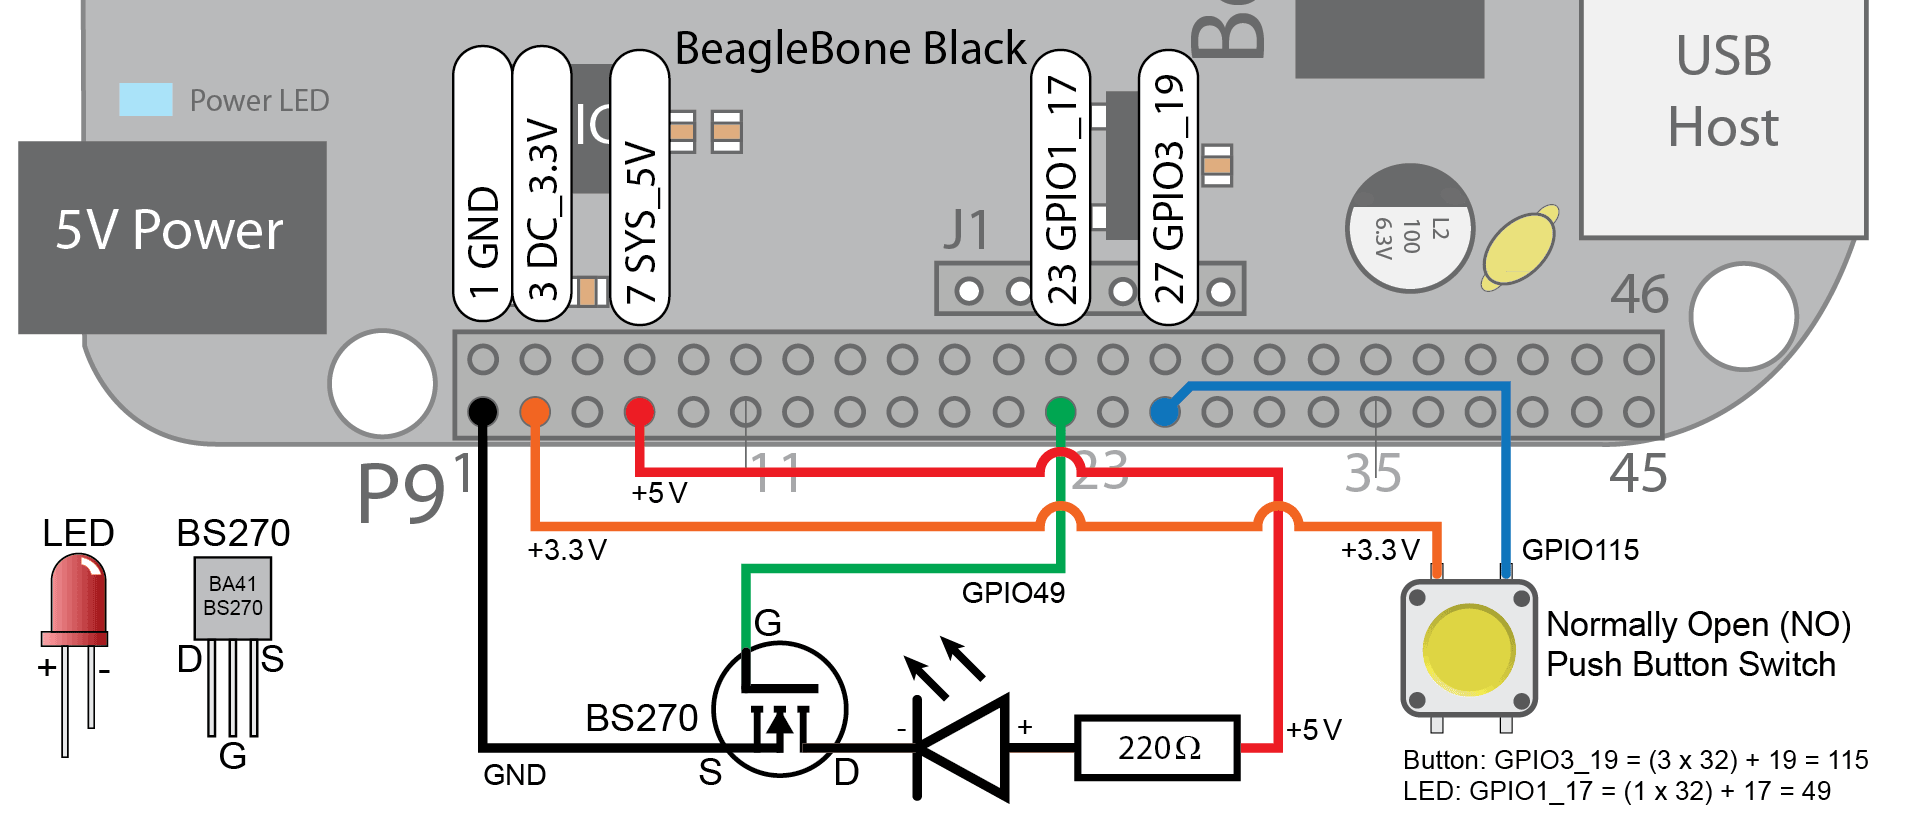
\includegraphics[width=0.875\textwidth]{Button-and-LED-large.png}
\end{center}
{\tiny \copyright \url[http]{derekmolloy.ie/kernel-gpio-programming-buttons-and-leds}}
\end{frame}




%\section{Aufgaben}

\begin{frame}{Ziel}
 \begin{itemize}
  \item \cod{hello-world} auf dem \host und auf dem \targetS
  \item \cod{primes} auf dem \host und auf dem \targetS
 \end{itemize}
\end{frame}


\begin{frame}{The big Picture}
 \begin{itemize}
  \item Source File: \cod{hello-world.cc}
  \item falls es nicht klapt ?
  \begin{itemize}
   \item wo ist der File ?
  \end{itemize}
 \end{itemize}
\end{frame}


%\subsection{Die Programme}
%\begin{frame}{Development}{\cod{hello-world-c.c}}
%\hspace*{-8mm}
%{
%\begin{tabular}{llllll}
% Host & Target & OS & Toolchain & Verbindung & Bemerkungen\\
% \hline
% \targetS & \targetS & Debian & mitgeliefert&&\\
% \host   & \targetS & Debian & \cod{\tiny tc-tinl-gcc-8.1.0-2018.05.21.tar.gz} & sshfs\\
% \host   & \targetS & minimal & \cod{\tiny tc-tinl-gcc-8.1.0-2018.05.21.tar.gz} & SD-Card  &später\\
% \host   & \targetS & minimal & \cod{\tiny tc-tinl-gcc-8.1.0-2018.05.21.tar.gz} & curlftpfs&später\\
%\end{tabular}
%}
%\remark{Toolchain auf der Cloud: \href{https://drive.switch.ch/index.php/s/A6H382zEGDrgfAL}
%       {\Huge tinL}}
%\end{frame}




\end{document}

